% !TeX spellcheck = en_US
\section*{Test run of detmsnn.py}

Test report

by E. Marquer, 2018/05/16, Synalp and Université de Lorraine

\subsection{Abstract}

Performance test of the `cat' (concatenated) output strategy compared to
the `add' strategy. Test to do a run on 4 epochs, with GPU, of the basic
model of MSNN, with concatenated output strategy.

\subsection{Paradigm}

This test run of \emph{detmsnn.py}, with INFO level log output, loss per
percentile and vbpc per epoch, is executed with \emph{cuda}, for 4
epochs.

The test is done with branch
\href{https://gitlab.inria.fr/emarquer/awd-lstm-lm/tree/growing}{growing},
an allocated time of 24h, not interactive

\textbf{/!\textbackslash{} Had to reduce evaluation courpus size down to
1/1000, to reduce computation time while keeping a big enough corpus to
compute BPC /!\textbackslash{}}

\newpage
\subsubsection{Hyperparameters}

\begin{longtable}[]{@{}ll@{}}
\hline
Hyperparameter & Value\tabularnewline
\hline
\endhead
nhidden & 920\tabularnewline
embedsize & 400\tabularnewline
bptt & 200\tabularnewline
batch\_size & 1\tabularnewline
eval\_batch\_size & 1\tabularnewline
lr & 0.001\tabularnewline
wdecay & 1.2e-06\tabularnewline
cuda\_on & True\tabularnewline
log\_interval & 100\tabularnewline
nepochs & 4\tabularnewline
max\_seqs & 5\tabularnewline
\hline
\end{longtable}

\subsubsection{Node}

OAR\_JOB\_ID=1563805 with GPU grimani-1

Job start time: 2018-05-16 08:53:20

Estimated job stop time: 2018-05-17 08:53:20

Command used:

\begin{lstlisting}[language=bash]
oarsub -q production -p "GPU <> 'NO'" -l "nodes=1,walltime=24:00:00" "bash runmsnn.sh"
\end{lstlisting}

Status verification loop:

\begin{lstlisting}[language=bash]
let x=0; while [ "true" ]; do echo "$x" $(oarstat -s -j 1563805); let ++x; sleep 120; done
\end{lstlisting}

\subsection{Results}

Total run time for 4 epochs: with real stop time of 08:53:28, the total
run time of the training is approximately 24h, with only 22\% of one
epoch done, and a final Validation BPC of 3.57.

Estimated run time for a full epoch: 24h / 22\% \textasciitilde{}=
109h/epoch. This corresponds to 436h for a 4 epoch run, and this is
critical.

The `cat' strategy is way more efficient in corpus consumption, even if
it is dramatically slower than the additive strategy.

\subsubsection{Comparative analysis}

The comparative plot shows that with the `cat' strategy, BPC diminution
is way faster than with the additive strategy. Computation-time wise, it
is obvious that the `cat' strategy is slower, with ??h/epoch, than the
`add' strategy, with 50min/epoch. This difference is too large to be due
to the device alone.

\begin{figure}[h]
\centering
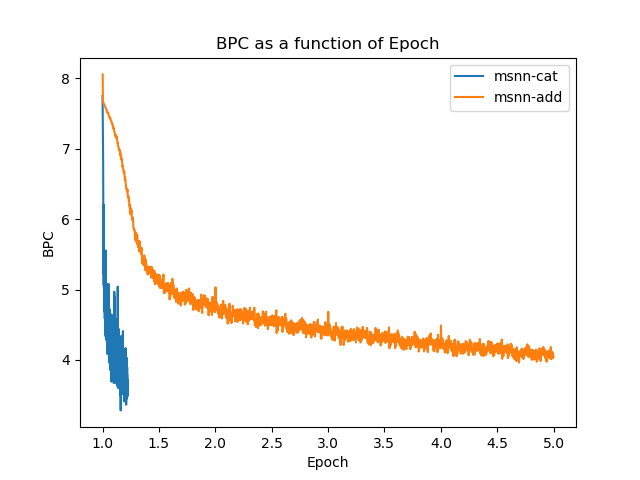
\includegraphics{parts/appendix/reports-gmsnn/docs_esteban-latex/test_reports/comparative-bpc-msnn-det-msnn-cat.png}
\caption{Comparative BPC}
\end{figure}

\subsubsection{Plot}

\paragraph{BPC/fraction of corpus}

BPC: BPC per fraction of the corpus (an interval of 1 correspond a
complete corpus, or an epoch).

Validation BPC: BPC per fraction of the corpus, on the validation
corpus.

Layers: Number of layers per fraction of the corpus.
\begin{figure}[h]
	\centering
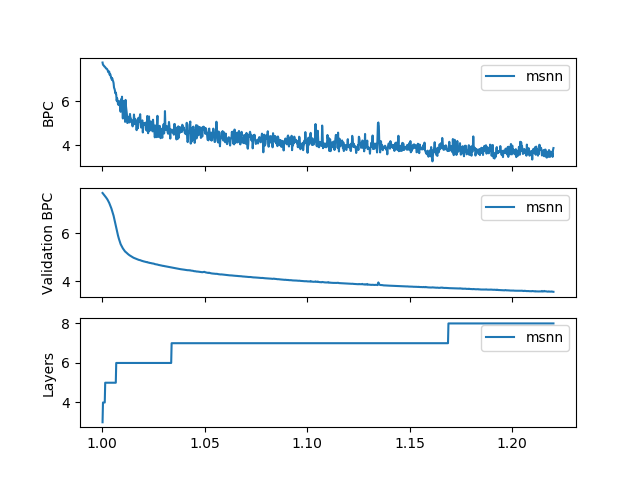
\includegraphics{parts/appendix/reports-gmsnn/docs_esteban-latex/test_reports/msnn-4/2018_05_17-13h49.png}
\caption{Comparative BPC}
\end{figure}

\newpage
\subsection{Potential ameliorations \& next steps}

Next step is to try to reduce run time.
